% 3.3.BuildApplication.tex
%	Last update: 2019/10/07 F.Kanehori
%newpage
\subsection{R8w47HeMnww1Wqw5}
\label{subsec:BuildApplication}

\noindent
\KLUDGE アプリケーションのビルドは従来と変わりがありませんが、
\KLUDGE ソリューションに新しいターゲット
\tt{ALL\_BUILD}, \tt{sync}\KLUDGE が追加されています。
\KLUDGE ここでは、これらについて説明します。

\medskip
\noindent
\tt{ALL\_BUILD}
\begin{narrow}[20pt]
	\KLUDGE これは\cmake \KLUDGE が自動的に作成するターゲットでmake all\KLUDGE に相当するものと
	\KLUDGE されています。ただしVisual Studio\KLUDGE 上ではALL\_BUILD\KLUDGE の依存関係の設定が不正確で、
	\KLUDGE このターゲットをビルドしても正しい結果は得られないようです。
	{\bf{\KLUDGE このターゲットは無視してください}}
\end{narrow}

%\noindent
%\tt{RunSwig\_Clean} \\
%\tt{EmbPython\_RunSwig\_Clean}
%\begin{narrow}[20pt]
%	\KLUDGE 従来の方法では、ターゲットRunSwig\KLUDGE は\KQuote{\KLUDGE メイクファイルプロジェクト}\KLUDGE として
%	\KLUDGE 作成されており、このターゲットには\KQuote{\KLUDGE ビルド}, \KQuote{\KLUDGE リビルド},
%	\KQuote{\KLUDGE クリーン}\KLUDGE のそれぞれに対して別々に適切なコマンドを設定することが
%	\KLUDGE できました。
%	\KLUDGE しかし\cmake \KLUDGE では、
%	\KLUDGE 残念ながら\KQuote{\KLUDGE メイクファイルプロジェクト}\KLUDGE を作成することができず、
%	\KLUDGE 全体を\KQuote{\KLUDGE リビルド}\KLUDGE しようとてもRunSwig\KLUDGE だけは\KQuote{\KLUDGE リビルド}\KLUDGE されません。
%	\begin{narrow}[s][15pt]
%		\KLUDGE これは、\cmake \KLUDGE で作成されたRunSwig\KLUDGE ターゲットは
%		\KLUDGE カスタムビルドコマンドを実行するためのターゲットで、
%		\KLUDGE ここで設定されているコマンドは
%		\KQuote{\KLUDGE ビルド}\KLUDGE 時にしか実行されないためです。
%	\end{narrow}
%	\KLUDGE したがって、
%	{\bf{\KLUDGE 全体を(\KLUDGE もしくはRunSwig\KLUDGE を)\KQuote{\KLUDGE リビルド}\KLUDGE しようとするときは、
%	\KLUDGE その前に必ずRunSwig\_Clean\KLUDGE ターゲットを\KQuote{\KLUDGE ビルド}\KLUDGE する必要があります。}}
%	\KLUDGE 一手間増えますが、忘れないようにしてください。
%	{\bf{EmbPython\_RunSwig\_Clean\KLUDGE についても同様です。}}
%\end{narrow}

\noindent
\tt{sync}
\begin{narrow}[20pt]
	\KLUDGE これは\KQuote{\ref{subsec:CmakeApplication} cmake\KLUDGE の実行}\KLUDGE で述べたとおり、
	\KLUDGE プロジェクトファイルの整合性を保つために作られたものです。
	\SprLib \KLUDGE のプロジェクトを一つでもビルドすれば
	\KLUDGE このターゲットは必ず最初に実行されますから、
	\KLUDGE このターゲットに対して何らかのアクションを起こす必要はないでしょう。
\end{narrow}

\bigskip
\bigskip
\noindent
\thinrule{\linewidth}
\noindent
\bf{\KLUDGE 補足}\KLUDGE  
\begin{narrow}
	\bf{2019/9/30 (commit 1d8e5ce)\KLUDGE 以前に配布した\CMakeLists{.*.dist}\KLUDGE を元に
	\CMakeLists{}\KLUDGE を作成して使用している場合}

	\medskip
	RunSwig\KLUDGE でclean/rebuild\KLUDGE の対応ができていなかったため、
	clean\KLUDGE と同等の機能を実現するためのターゲットRunSwig\_Clean\KLUDGE が作成されて
	\KLUDGE いるはずです。

	\KLUDGE 上記日付以降の\SprLib \KLUDGE をダウンロードし\cmake \KLUDGE を実行していただければ、
	RunSwig\KLUDGE はclean/rebuild\KLUDGE 対応となります。
	\KLUDGE ただし、RunSwig\_Clean\KLUDGE をビルドすると
	\begin{narrow}
	\tt{python: can't open file '.../Clean.py': ... No such file ...}
	\end{narrow}
	\KLUDGE というエラーが起きます。実害はありませんがRunSwig\KLUDGE のclean\KLUDGE は行なわれません。

	\medskip
	\KLUDGE  RunSwig\_Clean\KLUDGE ターゲットを生成されないようにするには、
	\KLUDGE 新しい配布ファイルから\CMakeLists{}\KLUDGE を再作成するか、
	\KLUDGE または既存の\CMakeLists{}\KLUDGE から以下の部分を削除して再\cmake \KLUDGE してください。

	\begin{narrow}\begin{figure}[h]
	    \begin{narrow}[30pt]
		\begin{center}\fbox{%
		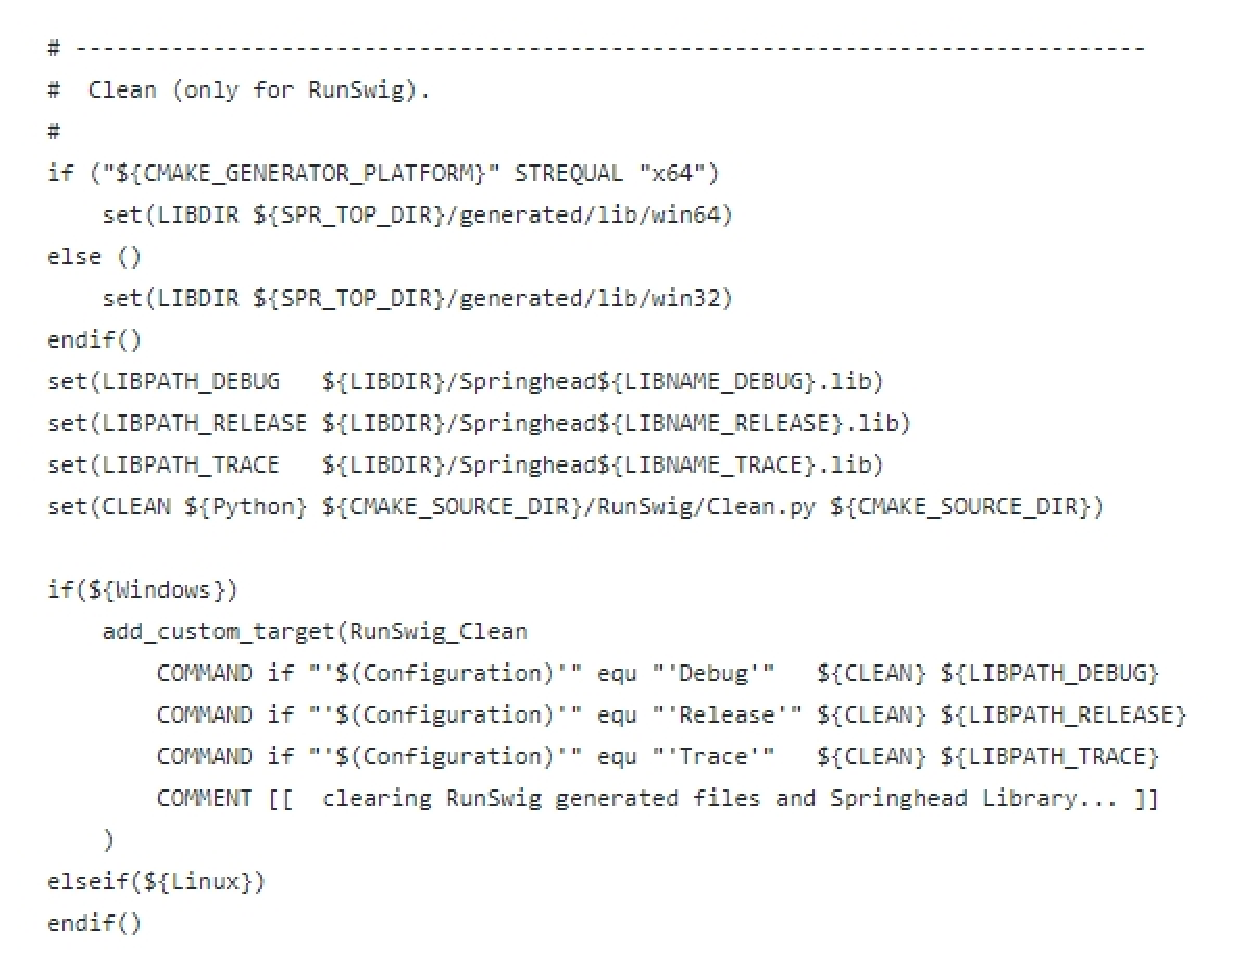
\includegraphics[width=.8\textwidth]{fig/RemoveRunSwigClean.eps}
		}\end{center}
		\label{fig:SpringheadLibraryTree}
	    \end{narrow}
	\end{figure}\end{narrow}
	
	EmbPython\_RunSwig\_Clean\KLUDGE についても同様です。	
	
\end{narrow}

% end: 3.3.BuildApplication.tex
